\documentclass[10pt]{article}

% Sprachliche Besonderheiten %%%%%%%%%%%%%
\usepackage[ngerman]{babel} % Umlaute etc.
%\usepackage[english]{babel}
\usepackage[utf8x]{inputenc} % Input encoding des Dokuments
\usepackage[T1]{fontenc} % Font encoding des Dokuments
% %%%%%%%%%%%%%%%%%%%%%%%%%%%%

\usepackage[hyphens]{url}


% Ansprüche an mathematische und physikalische Notation %%%%%%%%%%%%%
\usepackage{amsfonts,amsmath,amsthm,amssymb} %% erweiterte Funktionalität für Formeln (Pakete der American Mathematical Society)
\usepackage[separate-uncertainty]{siunitx} %% vordefinierte Einheiten, einfaches Angeben von Einheiten (\SI{8 \pm 1}{cm}), die Unsicherheit soll mit +- abgetrennt werden, bei siuntix funktioniert babel leider nicht
%




% Tabellen %%%%%%%%%%%%%
\usepackage{microtype} %% optimiert das typographische Erscheinungsbild
\usepackage{enumitem} %% erlaubt Listen einfacher zu formatieren (bietet nosep für kompakte Listen)
\usepackage{ctable} %% erlaubt hübsche Tabellen über mehrere Seiten, beinhaltet booktabs (\toprule, \midrule, ...)
\usepackage{xcolor} %% ermöglicht farbigen Text ({\color{red} ...})
% %%%%%%%%%%%%%%%%%%




% Bilder %%%%%%%%%%%%%%%%%%%%%%%%%%%%%%%%%%%%%%%%%%%
%% erlaubt es Bilddateien einzubinden
%% (ctable graphicx intern auch. Trotzdem ist es sinnvoll graphicx expilizt zu laden.
%%  Sonst entstehen schwehr verständliche Fehler, wenn ctable entfernt wird)
\usepackage{graphicx}
\usepackage{wrapfig}
\usepackage{floatflt}
\usepackage{float} %% ermöglicht Bilder und Tabellen am eingegebenen Ort zu platzieren ([H])
\usepackage{subfig} %% ermöglicht Unter-Bilder in einer figure-Umgebung
%%\path{{img/}} %% Grafik-Dateien werden in den folgenden Ordnern gesucht
\DeclareGraphicsExtensions{.pdf,.png,.jpg} %% Grafikdateien haben die folgenden Endungen (höchste Priorität zu erst)
% %%%%%%%%%%%%%%%%%%%%%%%%%%%%%%%%%%%%%%%%%%%%%%%




% Layout und PDFLatex %%%%%%%%%%%%%%%%%%%%%%%%%%%%%%%%%%%%%%%%%%
\usepackage{parskip}                 %% Vertikaler Abstand zwischen Absätzen, Beginn eines Absatzes nicht einrücken
% \setlength{\parskip}{0.6em}   % Vertikaler Abstand zwischen Absätzen anpassen
% \setlength{\parindent}{0em}   % Einrück-Abstand anpassen

\usepackage[                             %% Seiten-Layout einstellen  
 a4paper,
 total={16cm,26cm},                  % Breite und Höhe des Inhalt-Bereichs
 top=20mm, left=30mm,            % Ränder oben und links
 headsep=10mm,                       % Abstand des unteren Rands der Kopfzeile vom oberen Rand des Inhalts
 footskip=10mm                        % Abstand des unteren des Inhalts zum oberen Rand der Fusszeile
]{geometry}
% %%%%%%%%%%%%%%%%%%%%%%%%%%%%%%%%%%%%%%%%%%%%%%%%%%%%%%%




% Links intern/extern %%%%%%%%%%%%%%%%%%%%%%%%%%%%%%%%%%%%%%%%%%
\usepackage[                            %% Ermöglicht Links im PDF, sollte möglichst spät in der Präambel geladen werden
 pdftex,                                    % wir verwenden pdftex/pdflatex
 bookmarks=true,                      % wir wollen auch im PDF-Reader ein Inhaltsverzeichnis
 bookmarksdepth=3,                 % das Inhaltsverzeichnis soll 3 Tiefen enthalten
 colorlinks=true,                        % Linktexte sollen Farbig sein
 linkcolor=black,                        % Links innerhalb des Dokuments bleiben schwarz
 citecolor=black,                       % Links zu Quellenangaben bleiben ebenfalls schwarz
 urlcolor=blue,                          % URL-Linktexte sollen blau dargestellt werden
%  pdfborder={0 0 0}               % Links im PDF erhalten keinen Rahmen, nur nötig wenn colorlinks=false
]{hyperref}

\usepackage[english, capitalise]{cleveref} % definiert \cref: Referenzen mit korrekter Bezeichnung (z.B. "Abbildung 1"), die Nummer alleine ist weiter mittels \ref verfügbar, muss NACH 'hyperref' geladen werden
%\usepackage[german]{cleveref}
% %%%%%%%%%%%%%%%%%%%%%%%%%%%%%%%%%%%%%%%%%%%%%%%%%%%%%%




% Anderes %%%%%%%%%%%%%%%%%%%%%%%%%%%%%%%%%%%%%%%%%%
\usepackage[final]{pdfpages} %% PDF einfügen 
\usepackage[final]{showkeys} %zeige Labels im Seitenrand. Dies ist praktisch um Verweise zu kontrollieren, die Option 'final' deaktiviert die Ausgabe von showkeys
% %%%%%%%%%%%%%%%%%%%%%%%%%%%%%%%%%%%%%%%%%%%%%%%
\usepackage[style=numeric,backend=biber]{biblatex}
\addbibresource{quellen.bib}




%% Angaben für \maketitle %%%%%%%%%%%%%
\title{Online Code Editor für C++}
\author{Nicola Krull}         
%%%%%%%%%%%%%%%%%%%%%%%%%%%%

%für bilder

%\usepackage{subcaption} 


%\usepackage[]{biblatex}
%\addbibresource{sources.bib}


\begin{document}
	
	\begin{titlepage}
	\begin{center}
	
	
	\huge
	\textbf{Online Code Editor für C++}
	
	\vspace{8cm}	
	
	\LARGE
	\textbf{Nicola Krull}
	
	\vspace{1cm}	

	\Large
	Maturaarbeit\\
	Betreut von
	Beni Keller
	
	\vspace{0.8cm}	

	 
	 Kantonsschule Zug\\
	 2019
	\end{center}
\end{titlepage}
	
	\tableofcontents
	\newpage
	
	\section{Einleitung}
	Online Editoren sind oft sehr nützlich. Mit einem Online Editor kann man sofort und von überall her loslegen. Man muss nicht zu erst den Editor und Compiler herunterladen und installieren, sondern man kann direkt vom Internet aus starten. Durch den Gebrauch eines Online Editor spart man Zeit und Speicherplatz. Deswegen ist die Programmierung eines Online Editors als Maturaprojekt eine interessante Wahl gewesen. Das Ziel des Projektes war es eine Webseite zu programmieren auf der man C++ Code schreiben und ausführen kann.
	
	Dabei lernt man vieles über Webseitenentwichlung wie zum Beispiel der Aufbau einer Webseite oder wie die Files miteinander kommunizieren. Man erkennt, dass viel Arbeit hinter den Element einer Webseite steckt. Es gibt ein Verständnis über die Prozesse die man durch einen einzigen Mausklick auslösst. Eine Webseite ist nicht so simpel wie sie aussieht.
	
	Das Hauptthema der Arbeit war, wie man die Webseite vor den Benutzern schützen kann. Durch das Sammeln von Information über Sicherheitsproblemen und Lösungsmethoden bekommt man nicht nur ein gutes Verständnis über Sicherheitsproblematiken sondern auch ein gutes Verständnis wie ein Computer aufgebaut ist. In der Arbeit werden Containers und virtuelle  Maschinen als zwei Mögliche Lösungsvorschläge dargestellt. Beides sind sehr bekannte Themen. Virtuelle Maschien werden heutzutage oft im Altag benutzt. Durch die Arbeit bekommt man ein genaueres Verständnis über Virtuelle Maschinen, was extrem interessant ist, denn viele Menschen benützen virtuelle Maschine, haben aber keine Ahnung was genau eine solche virtuelle Maschine macht.
	\pagebreak
	\section{Aufbau}
	\subsection{Design}
	Die Seite ist simpel aufgebaut. Es gibt eine Textbox in die man den C++ Code hineinschreibt und einen Submit Knopf. Sobald der Knopf gedrückt wird kommt man auf eine weitere Seite die entweder den Syntaxfehler oder die Antwort zurück gibt.
	\subsection{Software}
	Das Ziel des Projektes ist eine dynamische Webseite zu bauen. Eine dynamische Webseite ist eine Webseite bei welcher der Server mit der Webseite kommuniziert.\cite{dymWeb} % Ergänzung möglich  
	Für den Bau einer dynamischen Webseite benötigt man ein Webframework, welches die Interaktionen zwischen den 			Files steueren kann. Dafür wird das Webframework Express verwendet. Es ist ein serverseitiges Webframework, welches für die Plattform Node.js entwickelt wurde.\cite{express} Node.js ist eine open-source, serverseitige Plattform, welche JavaScript als Skriptsprache verwendet.\cite{nodejs}	Wenn man eine dynamische Webseite programmiert muss man immer zwischen serverseitigen und clientseitigen Code unterscheiden. Für die serverseitigen Programme wird für die Plattform grösstenteils Node.js verwendet und auf der Clientenseite läuft JavaScript, HTML und CSS. In diesem Projekt kommt grundsätzlich nur serverseitiger Programmstiel zur Anwendung. Um die graphischen Elemente auf der Website darstellen zu können, wird in diesem Fall die Templatesprache Jade verwendet. Sie ist zur Generierung von HTML-Seiten zuständig. Jade vereinfacht nicht nur die Syntax, sondern die funktioniert wie jede andere Programmiersprache, somit kann man für den HTML-Code Variabeln, If-Abfragen und for-Schleifen benützen. \cite{jade}

\begin{floatingfigure}[r]{11cm}
    \centering
    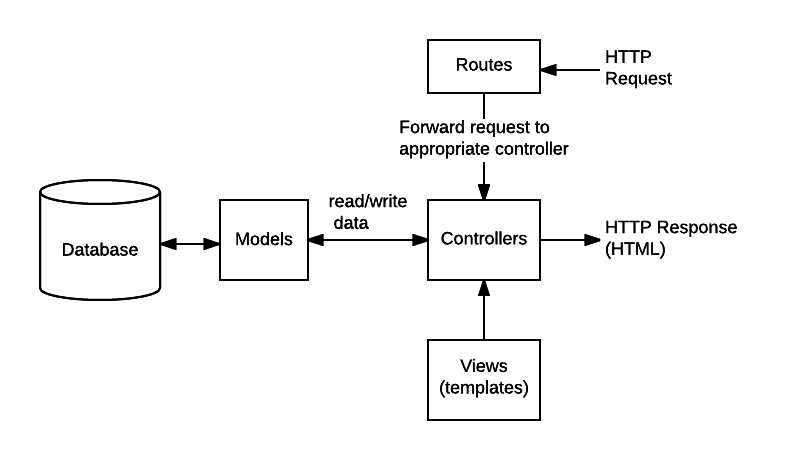
\includegraphics[width=10cm]{Bilder/MVCexpress.png}
    \caption{Express Aufbau \cite{exprRoutes}}
\end{floatingfigure}

Express kann man in die drei Teile, Views, Routes und Controllers aufteilen. In dem Views-Ordner sind die Jade Files gespeichert. Diese Dateien sind für das Design der Webseite zuständig. Wenn man beispielsweise eine Textbox und einen Button auf der Webseite sehen möchte, müsste man in einem Jade-File eine Textarea und einen Button kreieren. Wenn man nun etwas in die Textbox einsetzen und den Button drücken würde, würde die Website keine Reaktion zeigen. Es würde nichts geschehen da der Textinhalt weitergeleitet werden müsste und dazu noch keine Datei existiert. Dafür benötigt es die HTTP Methoden wie zum Beispiel GET und POST. Die Abkürzung HTTP steht für Hypertext Transfer Protokol und ist zuständig für die Kommunikation zwischen dem Client und dem Server.\cite{httpmethods} All diese HTTP Requests werden im Routes Ordner bearbeitet und zum Controllers-File weitergeleitet. In den Controllers-Files findet das Rechnen statt.  Alle benötigten Algorithmen befinden sich im Controllers Verzeichnis. Diese Algorithmen berechnen und führen alles aus, was der Server für die Website benötigt. Für dieses Projekt wäre, es das Compilieren von den Textdaten in der Textbox. Dafür wird die Bibliothek  Child Processes  von Node.js benutzt. Mit Child Processes können die Terminalbefehle automatisch ausgeführt werden und somit müssen diese nicht manuel eintippt werden. Da ich keine Datenbanken für diese Arbeit verwendet, ist der Gebrauch von Models vernachlässigbar. 

	
	\pagebreak
	\section{Security}
	\subsection{Sicherheitsprobleme}
		Ein Sicherheitsproblem bei der Webseite ist die Textbox. Ohne Sicherheitsmassnahmen würde die Webseite blindlings den Code, der in der Textbox geschrieben wurde, ausführen. Dies kann jedoch zu Problemen führen, denn der Compiler erkennt nicht ob der Code den Server schädigen könnte. 
		
		%\subsubsection{Zeit- und Platzkomplexität}
		Der User könnte Code schreiben welche die Laufzeit(Zeitkomplexität) oder den Speicherverbrauch(Platzkomplexität) zu stark auslastet. Wenn Informatiker Algorithmen programmieren, drücken sie den Algorithmus immer durch die  asymptotische Laufzeit und Speicherverbrauch  aus. Im Prinzip ist die asymptotische Laufzeit eine Abschätzung wie viele Rechenschritte der Computer ausführen muss. Dabei gibt es drei verschiedene Varianten zur Laufzeitabschätzung, die worst case-Laufzeit, die average case-Laufzeit und die best case-Laufzeit. Wie schon die englische Namen worst case- und best case-Laufzeit sagen rechnen sie die maximale und minimale Anzahl Rechenschritte aus. Bei der average case-Laufzeit wird die erwartete Laufzeit bei einer Gleichverteilung der Eingaben ausgegeben.\cite{laufzeit}  Man versucht nicht nur die Zeitkomplexität zu optimieren, sondern auch die Platzkomplexität. Bei der Platzkomplexität versucht man die Anzahl der Speicherzellen möglichst tief zu halten. Meistens verhalten sich die beiden Komplexitäten gegensätzlich. Dies bedeutet, dass man durch den Versuch der Optimierung der einen Komplexität, die andere möglicherweise verschlechtern wird.\cite{platzkomplexität} Man versucht daher die  Komplexitäten durch Funktionen, wie die nachstehende, asymptotisch abzuschätzen.	$$ O(f(n)) $$
		Das \textbf{n} steht für die Anzahl Eingaben und die O Notation benötigt man um die Funktion zu vereinfachen.\cite{Onotation} Zum Beispiel:
		$$ 3n^{3}+4n^{2}+10n+4 \in O(n^{3})$$
		Durch die O Notation kann man jede Laufzeit und Speicherverbrauch abschätzen. Es wäre praktisch wenn man jeden Code der geschrieben wird  auf Zeit- und Platzkomplexität analysieren könnte. Somit wüsste man wie stark der Server jeweils ausgelasstet werden würde. Ein solches Programm ist jedoch unmöglich zu kreieren. Der britische Mathematiker Alain Turing hatte das Halteproblem gelösst. Das Halteproblem befasst sich mit der Frage ob es möglich ist vorauszusagen ob ein Algorithmus jemals zu einem Ende gelangen würde. Alain Turing kam zum Schluss, dass es nicht möglich ist vorrauszusagen ob ein Algorithmus abbrechbend ist.\cite{halteproblem} Somit ist es auch nicht möglich seine Laufzeit abzuschätzen. Das selbe gilt auch für den Speicherverbrauch, denn Laufzeit und Speicherverbrauch verhalten sich equivalent. Dadurch wird jede einzelne nicht abbrechende Schlaufe zu einer Bedrohung. Deswegen müssen die verschiedenen Sicherheitsansätze einen Timer beinhalten der nach einer gewisssen Zeit den Prozess des Compilierens abbrechen würde.
		
	Ein weiteres Problem ist, dass man mit C++-Dateien auf die vollständige Umgebung des Servers zugreifen kann. Zum Beispiel mit dem C++ Befehl \textit{system()} kann man Befehle ausführen, welche man für den Terminal benützt. Für diesen Befehl müssen die Bibliotheken stdlib.h oder cstdlib zugriffsbereit sein.\cite{systemcpp} Dies bedeutet, dass der User alles auf dem Server verändern könnte, was nicht das Root Passwort benötigt. %Schlecht Formulieret
	Somit hätte der User fast vollständige Kontrolle über den Server.
	
	Durch die Textbox entstehen einige Sicherheitsprobleme. Der User der Website könnte die Laufzeit und Speicherkapazität des Servers überlasten. Dazu kommt, dass er auf die Daten welche auf dem Server gespeichert wurden, zugreifen könnte. Auch könnte er die Kontrolle des Servers übernehemen und für seine eigenen Zwecke nutzen oder einfach das Betriebssystem des Servers zerstören. Um alle diese Sicherheitsrisiken zu beseitigen, benötigt es eine Sicherheitssystem.
	
	\pagebreak
		
		
	\subsection{Mögliche Sicherheitsansätze}
	
		\subsubsection{Geplannter Ansatz}
	Ein mögliches Sicherheitssystem wäre ein Gebilde, welches die Dateiberechtigungen verändern würde und die eingehenden und ausgehenden Ports schliessen würde. In Unix Systemen kann man mit dem Befehl \textit{chmod}  die Berechtigungen von Ordnern und Dateien verändern. Dabei gibt es drei Gruppen: Eigentümer(user), Gruppe(group) und Sonstige(others). Für jede dieser Gruppen kann man drei verschiedene Grundrechte bestimmen. Das erste Recht \textbf{r} steht für den englischen Begriff read und bewirkt, dass man das Recht hat das File zu lesen. Das zweite Recht wird mit dem Buchstaben \textbf{w} ausgedrückt. Es steht für write und ermöglicht dem Benutzer Dateien zu schreiben. Das heisst er darf Dateien und Unterverzeichnisse erstellen, löschen, ändern und die Dateirechte der Unterverzeichnisse verändern. Das dritte und letzte Recht steht der Buchstabe \textbf{x} für execute. Diese Funnktion führt Dateien als Programme aus. Meist benutzt man eine Kombination der drei Berechtigungsfunktionen. Die einzelnen Berechtigungsfunktionen sind zu einer Zahl angeordnet. Das \textbf{x} ist gleich eins, das \textbf{w} hat den Wert zwei und das \textbf{r} den Wert vier. Wenn man eine kombination der drei Berechtigungen möchte muss man sie addieren. Im Falle, dass der  Benutzer alle Rechte haben soll, also lesen, schreiben und ausführen muss man die Berechtigung auf die Nummer sieben legen (1(\textbf{x}) + 2(\textbf{w}) + 4(\textbf{r}) = 7). 
	
	Das Ziel wäre einen Eingeschränkten User zu kreieren. Dafür muss man dem User für einige Ordner die Berechtigung verweigern. Dazu müsste man unter anderem die Ordner /sbin und /usr/bin für den User unzugänglich machen. Der Ordner sbin steht für die Englischen Wörter System Binaries. Auf Deutsch sind es die Systemprogramme, welche essentielle Aufgaben für die Systemverwaltung besitzen. Ausserdem sollte die Berechtigung auf die Konfigurationsdatei in /etc verboten werden. Hinzu kommen Einschränkungen der Berechtigungen von heiklen Programmen die sich im /bin und /usr/bin befinden.  Der /bin Ordner enthält unverzichtbare Programme. Der Unterschied zum /sbin ist, dass /bin von allen Benutzern benutzt werden kann. Im /usr/bin befinden sich Anwendungsprogramme unter anderem auch die Desktopumgebung.\cite{verzeichnis}
	
	Man muss alle nicht benötigten Ports schliessen. Dies gilt nicht nur für eingehende sondern auch für ausgehende Ports. Man schliesst die eingehenden Ports  wegen den Gefahren von ausserhalb. Die Schliessung von ausgehenden Ports ist wichtig, damit der Benutzer keine Daten nach draussen versenden kann. 
	
	\subsubsection{chroot}
	
	Chroot steht für 'change root'  und ist ein Programm welches das Rootverzeichnis für Unixsysteme ändern kann.\cite{chroot} Unix ist ein Betriebssystem, welches in den sechziger Jahren entwickelt wurde. Viele Betriebsysteme basieren auf Unixsysteme, so zum Beispiel das macOS, das iOS und die Linux Betriebsysteme. Dazu gehört auch das Betriebsystem Android.\cite{unix} Chroot generiert eine geschlossene Umgebung namens chroot jail. Diese Umgebung erlaubt den Zugriff auf  Files und Befehle ausserhalb dieses Ordners nicht. Somit kann der User nur auf diesen bestimmten Breich des Servers zugreifen und keinen Schaden am Server anrichten.\cite{archChroot}	
	
\pagebreak	
	
	\subsubsection{Containervirtualisierung}
	Containervirtualisierung ist ein Verfahren, welches sich auf eine Betriebssystemsfunktion bezieht, bei welcher der Kernel die Erstellung von multiplen isolierende User-Space Instanzen erlaubt. Diese erstellten Instanzen werden Containers gennant.\cite{OSlv} Ein Kernel ist die tiefste Softwareschicht eines Betriebsystems. Der Kernel ist zuständig für die Prozess- und Datenorganisation. Ausserdem kann der Kernel direkt auf die Hardware zugreifen.\cite{kernel} Die virtuelle Speicherverwaltung wird in User-Space und Kernel-Space unterteilt. Der User-Space ist der Ort an dem die  Anwendungssoftwaren ausgeführt werden. \cite{userSpace}
Der Unterschied zwischen einem Programm welches in einem Container und eines das von einem Betriebssystem ausgeführt wurde ist, der das Programm vom OS aus alle Elmente des Betriebssystems zur Verfügung hat, während das File im Container nur auf die Informationen innerhalb des Containers zugreifen kann. Da man komplett isoliert ist muss man einige Elemnte wie zum Beispiel Bibliotheken für die Programme, die in diesem Container ausgeführt werden, hinzufügen. 
Für unixartige Systeme sind Containers fortgeschrittene Implementierungen von chroot. \cite{OSlv}
	
	Eine Containervirtualisierungstechnologie ist Linux Containers(Abkürzung LXC). Es ist ein Verfahren, welches eine Virtualisierung von Softwaren auf Betriebssystemebene innerhalb des Linux-Kernels generiert. 
Das Besondere an den Linux Containers ist, dass sie im Vergleich zu herkömmlichen Virtuellen Maschinen, wie zum Beispiel VMWare oder KVM, einzelne Anwendungen in virtuellen Umgebugen ausführen können. Ausserdem ist es möglich ein ganzes Betriebssystem in einem solchen Container zu starten.  \cite{lxc}
%Es gibt zwei Arten von Linux Containers die \textit{privileged Containers} und die \textit{unprivileged Containers}. Die \textit{privileged Containers} sind nicht 

\begin{figure}[h!]
    \centering
    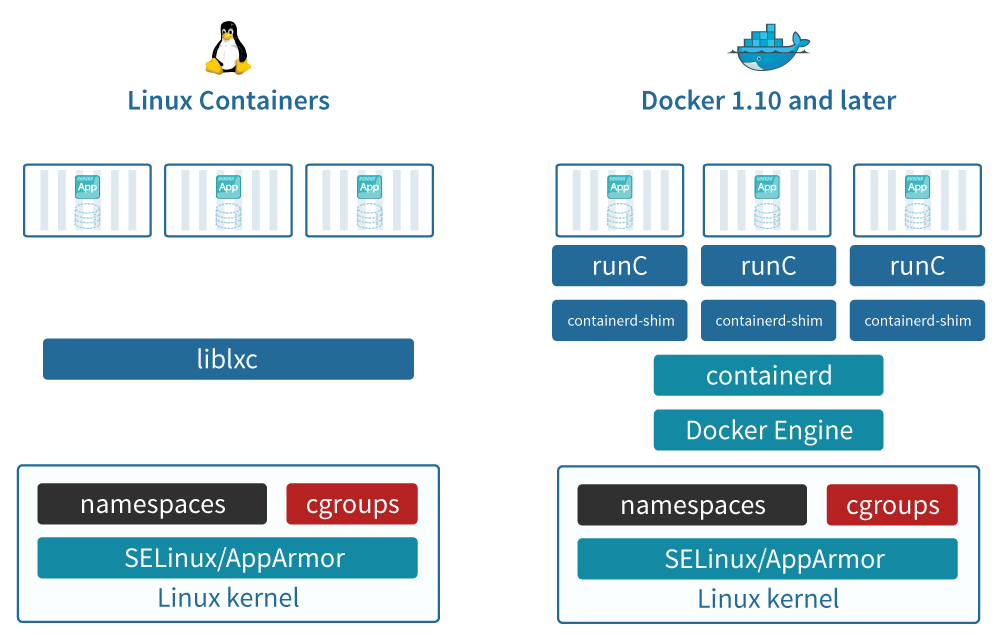
\includegraphics[width=12cm]{Bilder/ContainerArchitektur.png}
    \caption{Architektur von zwei Containertechnologien \cite{container}}
\end{figure}


Eine weitere Containervirtualisierungstechnologie ist Docker. Docker ist eine der bekanntesten Containervirtualisierungsarten. Früher basierte er auf dem LXC System. Man stellte dies jedoch ein und ersetzte den Teil der auf dem LXC System basierte, durch eine eigene Implementierung names libcontainer. Im Grunde ist es die Bibliothek liblxc die durch den libcontainer ersetzt wurde.\cite{container} Liblxc ist eine Bibliothek welche für die Kommunikation zwischen Kernel und Container zuständig ist.\cite{liblxc} 

Im Linux Kernel sind praktisch alle Containertechnologien gleich aufgebaut. Dazu gehören die Kernel-Funktionen cgroups und Namespaces. Cgroups, auch Control Groups genannt, ist ein Verfahren welches die Ressourcen verwaltet. Diese Systemsoftware führt dazu, dass der Container nur eine begrenzte Menge an Speicher, Rechenleistung und Disk I/O zur Verfügung hat. Sonst würde er die ganzen Ressourcen für sich alleine beansprechen. Unter Disk I/O versteht man die Eingabe(Input) und Ausgabe(Output), die Vorgänge einer physischen Festplatte. Wenn man eine Datei von der Festplatte lesen möchte muss der Prozessor warten bis die Datei gelesen wurde. Das Selbe gilt auch fürs Schreiben. \cite{diskIO} Die Systemsoftware Namespace benötigt man um die Prozesse eines Containers zu verbergen. Ansonsten könnte man über einen weiteren kreierten Container Informationen über die Prozesse eines anderen Containers erhalten.\cite{cgroupsNamespace} SELinux und APPArmor sind Mandatory Acces Control(MAC) Systeme. MAC Systeme sind zuständig für Zugriffe von Benutzern und Prozessen auf einzelne Objekte. Wenn ein Zugriff nicht erlaubt ist, wird er vom MAC System unterbunden.\cite{MAC} 

\pagebreak



Eine wichtige Funktion hat die Docker Engine. Sie kreiert und führt Docker Containers aus.\cite{Engine} Die Engine ist eine client-server Applikation.\begin{floatingfigure}[r]{12cm}
    \centering
    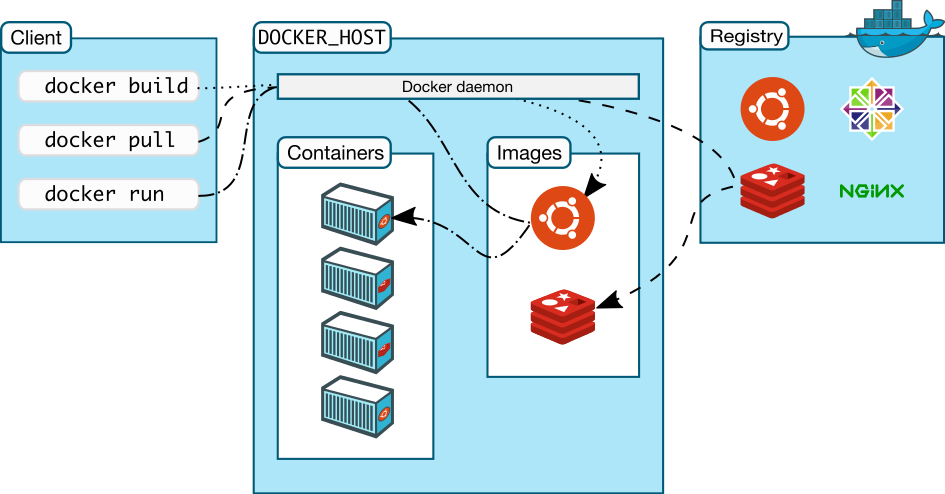
\includegraphics[width=12cm]{Bilder/docker.png}
    \caption{Docker Architektur \cite{dockerEngine}}
\end{floatingfigure} Man kann sie in drei Teile aufteilen, der Docker Daemon, die Docker API und der Docker CLI. Der Docker Daemon ist ein Programm welches auf die Anfragen der Docker-API wartet. Ausserdem kommuniziert er mit anderen Daemons und verwaltet die Docker Objekte wie Images, Containers, Netzwerke und  Volumes. Unter dem Begriff Docker Image versteht man ein read-only template welche Anweisungen zur Erstellung eines Docker Containers besitzt.\cite{dockerEngine} Read-only ist die Bezeichnung für Objekte oder Konstrukte welche nach dem kreieren nicht mehr veränderbar sind. Man kann sie nur noch lesen.\cite{readOnly} Wenn ein Container erstellt wird, werden Volumes initialisiert. Diese Volumes besitzen Funktionen welche für das Persistieren und Teilen der Daten zuständig sind.\cite{volumes} Der Docker Client kann mit dem Daemon kommunizeiren indem sie die Docker API verwenden. 

% Unter den Wörter Docker Image versteht man eine Datei, welche Code innerhalb eines Containers ausführt./cite[image] 
 %Wenn der Docker User ein Image ausführt, wird es zu einer oder mehreren Instanzen des Containers. 



\pagebreak

\subsubsection{Hypervisor}
Bei Hypervisoren, auch Virtual Machine Monitor gennant, handelt es sich um eine Software, welche virtuelle Maschinen von eiem beliebigen Betriebssystem aus starten kann. Es gibt zwei Arten von Hypervisoren.  \cite{hypervisor}


\begin{figure}[H]%ABbildungsverzeichniss link https://www.crisp-research.com/was-ist-ein-hypervisor/ und datum noch hin
  \centering
  \begin{minipage}[H]{0.4\textwidth}
    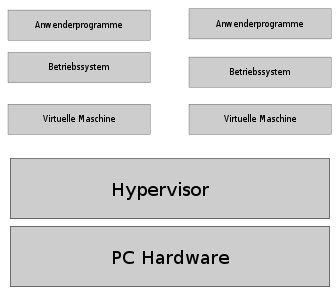
\includegraphics[width=\textwidth]{Bilder/hypervisorTyp1.jpg}
    \caption{Typ-1-Hypervisor}
  \end{minipage}
  \hfill
  \begin{minipage}[H]{0.4\textwidth}
    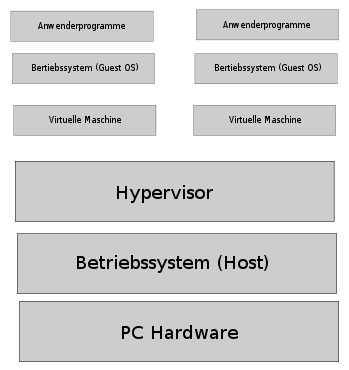
\includegraphics[width=\textwidth]{Bilder/hypervisorTyp2.jpg}
    \caption{Typ-2-Hypervisor}
  \end{minipage}
\end{figure}
	
	Der Typ-1-Hypervisor auch native oder bare-metal Hypervisor genannt läuft direkt auf der Hardware und benötigt passende Treiber. Dieser Hypervisor benötigt keine vorherige Betriebssystem-Installation. 
	Der Typ-2-Hypervisorbraucht ein vollständiges Betriebssystem auf dem Hostsystem. Es nutzt die Gerätetreiber des Benutzersystems für den Zugriff auf die Hardware des Hostsystems. 
	
	Das benutzen eines Hypervisor ist ein möglicher Sicherheitsansatz, da er virtuelle Umgebungen kreieren kann. Die Vorteile von diesen virtuellen Umgebungen sind, dass sie vollstäding isoliert sind und man immer wieder ein weiteres Betriebssystem kreieren oder löschen kann. Somit würde man ein Shell-Script schreiben, welches automatisch pro User eine virtuelle Umgebung kreiert. In dieser Umgebung würde dann auch die Compilierung stattfinden. Da es in einem virtuellen Betriebssystem stattfinden würde, würde nichts kaputt gehen. Nach dem Kompilieren, würde das Betriebsystem den Output in einen Ordner legen welcher das Hostsystem mit dem virtuellen Betriebsystem teilt. Sobald Output übermittelt wurde, wird das virtuele Betriebssystem gelöscht.
	
	Ein möglicher Hypervisor ist der KVM. Es steht für Kernel-based Virtual Machine. Der KVM ist seit 2007 in den Linux Betriebtssysteme im Haupt-Kernel integriert. % KVM konviert das Linuxbetriebsystem in ein bate-metal Hypervisor (Typ 1). 
	Damit es die Virtualisierung unterstützt muss es auf der x86 Hardware installiert sein.
	
	Ein wichtiges Element für Hypervisoren ist libvirt. Libvirt ist eine Bibliothek welche die Verwaltung von virtuelle Maschinen auf einem Hostsystem zuständig ist. Man kann libvirt unteranderem für den KVM Hypervisor gebrauchen. /cite{libvirt}  Man kann es aber auch für den Container LXC verwenden.
	%https://www.redhat.com/de/topics/virtualization/what-is-KVM link
	

	\pagebreak
	\section{Erweiterungsmöglichkeiten}
	Eine der nützlichsten Erweiterungsmöglichkeiten wäre sicherlich, dass der Output in einer bearbeitbaren Textbox gedruckt werden könnte. Es ist nicht möglich den Eingabebefehl (in C++ wäre es \textit{cin}) zu benutzen. Bis jetzt muss man die Eingabe als Variabeln selbst in den Code hineinschreiben. 
	
	Eine weitere Erweiterung wäre die Erstellung eines Einlogsystem. Somit könnte man den selbst geschriebenen Code direkt auf dem Server speichern. Dafür wäre der Einsatz einer Datenbank nötig. Dies sollte keine Schwierigkeiten bereiten, denn Express hat schon eine Schnittstelle für Datenbanken. Somit könnte man auf geschriebene Algorithmen und auf solche die noch in Arbeit sind von überall her zugreifen. 
	
	Mit einem Accountsystem gibt es weitere unzählige neue Möglichkeiten. Eine dieser Möglichkeiten wäre ein System zu programmieren bei dem es möglich wäre gleichzeitig von zwei verschiedenen Accounts aus die selbe Datei zu bearbeiten. Man könnte Gruppen bilden welche an einem Projekt arbeiten könnten. Dazu würde ein Chatsystem kommen in dem man miteinander kommunizieren kann und Programme austauschen könnte. Das Ziel wäre eine Website zu gestallten welche die Programmierer näher zusammenzubringen würde.   
	 
	
	
	\pagebreak
	\listoffigures
	
	\printbibliography
	\begin{thebibliography}{999}
\bibitem{dymWeb} 
\url{https://blog.kompaktdesign.com/webdesign/statisch-vs-dynamisch/} \bigskip 30.12.2018
 
\bibitem{express} 
\url{https://de.wikipedia.org/wiki/Express.js} \bigskip 25.10.2018
 
\bibitem{nodejs} 
\url{https://de.wikipedia.org/wiki/Node.js} \bigskip 25.10.2018

\bibitem{jade}
\url{https://t3n.de/news/jade-638027/} \bigskip 25.10.2018

\bibitem{exprRoutes}
\url{https://developer.mozilla.org/en-US/docs/Learn/Server-side/Express_Nodejs/routes} \bigskip 19.01.2019
%%felhler bei hyperlink

\bibitem{httpmethods}
\url{https://www.w3schools.com/tags/ref_httpmethods.asp}%link geht noch nicht
 \bigskip 25.10.2018
 
 \bibitem{chroot}
 \url{https://en.wikipedia.org/wiki/Chroot} \bigskip 30.12.2018
 
 \bibitem{unix}
 \url{https://de.wikipedia.org/wiki/Unix} \bigskip 30.12.2018
 
 \bibitem{archChroot}
 \url{https://wiki.archlinux.org/index.php/Chroot} \bigskip 30.12.2018
 
 \bibitem{OSlv}
 \url{https://en.wikipedia.org/wiki/Operating-system-level_virtualization} \bigskip 30.12.2018
 %link geht noch nicht
 
 \bibitem{kernel}
 \url{https://de.wikipedia.org/wiki/Kernel_(Betriebssystem)} \bigskip 30.12.2018

\bibitem{container}
	 \url{https://robin.io/blog/containers-deep-dive-lxc-vs-docker-comparison/} \bigskip 23.01.2019
	 
\bibitem{diskIO}
	 \url{http://blog.scoutapp.com/articles/2011/02/10/understanding-disk-i-o-when-should-you-be-worried} \bigskip 23.01.2019
	
\bibitem{cgroupsNamespace}
	 \url{https://jaxenter.de/docker-einfuehrung-linux-basics-62049/6} \bigskip 23.01.2019

\bibitem{MAC}
	 \url{https://www.admin-magazin.de/Das-Heft/2009/03/Mandatory-Access-Control-mit-Smack} \bigskip 23.01.2019

\bibitem{userSpace}
	\url{https://en.wikipedia.org/wiki/User_\space} \bigskip 31.12.2018 %look if \- works

\bibitem{lxc}
	 \url{https://www.webhod.de/lxc-und-lxd-was-sind-linux-container} \bigskip 30.12.2018 

\bibitem{hypervisor}
	\url{https://www.searchdatacenter.de/definition/Hypervisor-Virtual-Machine-Monitor-VMM} \bigskip 10.01.2019

\bibitem{liblxc}
	\url{https://www.sdxcentral.com/cloud/containers/definitions/what-is-a-linux-container/} \bigskip 26.01.2019

\bibitem{dockerEngine}
	\url{https://docs.docker.com/engine/docker-overview/} \bigskip 26.01.2019

\bibitem{Engine}
	\url{https://www.quora.com/What-is-docker-engine} \bigskip 26.01.2019

%\bibitem{image}
%	\url{https://searchitoperations.techtarget.com/definition/Docker-image} \bigskip 27.01.2019


\bibitem{readOnly}
	\url{https://www.techopedia.com/definition/856/read-only} \bigskip 27.01.2019

\bibitem{laufzeit}
	\url{http://www.uni-protokolle.de/Lexikon/Asymptotische_Laufzeit.html} \bigskip 29.01.2019
	

\bibitem{platzkomplexität}
	\url{https://www.leda-tutorial.org/de/offiziell/ch02s02s03.html} \bigskip 29.01.2019
	
\bibitem{Onotation}
	\url{https://soi.ch/wiki/algorithms-intro/} \bigskip 30.01.2019

\bibitem{systemcpp}
	\url{https://www.geeksforgeeks.org/system-call-in-c/} \bigskip 30.01.2019
	
\bibitem{halteproblem}
	\url{https://de.wikipedia.org/wiki/Halteproblem} \bigskip 01.02.2019
	
\bibitem{verzeichnis}
	\url{https://wiki.ubuntuusers.de/Verzeichnisstruktur/} \bigskip 30.01.2019
	
\bibitem{volumes}
	\url{https://jaxenter.de/einfuehrung-docker-tutorial-container-61528} \bigskip 30.01.2019	

\bibitem{libvirt}
	\url{https://de.wikipedia.org/wiki/Libvirt} \bigskip 30.01.2019	
%%	\printbibliography 
%%	\listoffigures
\end{thebibliography}

\end{document}
